\documentclass[a4paper,12pt]{report}

\usepackage{alltt, fancyvrb, url}
\usepackage{graphicx}
\usepackage[utf8]{inputenc}
\usepackage{float}
\usepackage{hyperref}

\usepackage[italian]{babel}

\usepackage[italian]{cleveref}

\title{\textbf{Elaborato per il corso di Basi Di Dati \\ A.A 2022/2023}}

\author{Ettore Farinelli \\ ettore.fainelli@studio.unibo.it \\ 0001019995}

\date{\today}

\begin{document}

\maketitle

\tableofcontents

\chapter{Analisi dei requisiti}
Si pone l'obbiettivo di realizzare un database capace di gestire un organizzazione di arti marziali come può essere, 
per esempio, \textsc{L'Ultimate Fighting Championship, (UFC)}. La base di dati dovrà quindi essere capace di registrare 
nuovi \textbf{lottatori} e in caso rimuoverli(squalifica, infortuneo, ritiro). Inoltre sarà possibile registrare \textbf{eventi}, 
dove i combattenti si scontreranno aggiornando (dopo gli \textbf{scontri}), gli \textbf{score} dei partecipanti 
e in caso le \textbf{classifiche}.

\section{Intervista}
A seguito di una prima intervista si sono ottenute le seguenti richieste:\medskip

Per ogni partecipante alla lega bisogna tenere traccia del nome, cognome, codice fiscale, data di nascita, peso e \textbf{arte 
marziale} in cui vuole lottare (più possibilità disponibili). Alla iscrizione di un nuovo lottatore esso verrà inserito all'ultimo 
posto nella classifica della propria categoria, e dovrà effettuare almeno un combattimento all'anno, oppure verrà  
squalificato dalla lega. Ci sarà la possibilità di registrare i \textbf{team} dei combattenti tenendo traccia di: nome, amministratore e 
origine. Saranno presenti diverse classifiche per ogni tipo di categoria dove i lottatori saranno ordinati 
in base ai loro \textbf{record} (V, P, S), dove le vittorie assegnano 3 punti, i pareggi 1 e le sconfitte 0.\par
Le categorie in cui verranno suddivisi i membri della lega sono: \textit{Peso Piuma} (fino a 65kg), \textit{} 
(65kg - 77kg), \textit{Peso Medio} (77kg - 84kg) e \textit{Pesi Massimi} (da 84kg in poi). Inoltre ci sarà una divisione in 
arti marziali: \textit{MMA} (Mixed Martial Arts), \textit{BJJ} (Brazial Jiu Jitsu) e infine \textit{Muay Thai}. Per ogni 
partecipante dovranno essere inserite le discipline di competenza possibilmente modificabili in futuro (sarà gestito in maniera 
analoga il peso). Inoltre, partecipanti appartenenti a una determinata categoria potranno scontrarsi solo con altri membri 
della stessa. Gli eventi saranno constituiti da almeno 2 combattimenti ciascuno, bisognerà tener traccia del: nome dello stadio, 
luogo (indirizzo), costo noleggio stadio, spesa staff, data, orario inizio, orario fine, biglietti standard venduti, biglietti 
premium venduti, introiti netti, inoltre sarà necessario poter associare a un evento degli sponsor selezionabili tra quelli disponibili 
che hanno effettuato un contratto con la lega. Ogni lottatore partecipante riceverà un pagamento extra e verrà calcolata una quantità di guadagni 
tramite pubblicità, tutto in base al numero di biglietti venduti per l'evento, così da poter calcolare gli introiti dell'evento, 
il quale verrà aggiunto in una \textsc{History} dove si potranno visualizzare tutti gli eventi passati, 
avendo infine la possibilità di visualizzare i guadagni e le spese totali della lega.

\section{Definizioni}
\begin{itemize}
    \item \textbf{Lottatore}: partecipante alla lega.
    \item \textbf{Organizzatore}: amministratore che ha l'accesso al database e le autorizzazioni per gestirlo. 
    \item \textbf{Evento}: un insieme di scontri avente un luogo e una data.
    \item \textbf{Scontro}: un incontro tra due lottatori della stessa categoria.
    \item \textbf{Classifica}: lista numerata in ordine dal partecipante migliore al peggiore in base ai record personali.
    \item \textbf{Arte marziale}: disciplina frequentante da un partecipante.
    \item \textbf{Team}: associazione a cui possono far parte 1 o piu combattenti, ha lo scopo di seguirli durante gli scontri e allenarli.
    \item \textbf{Record}: terna di vittorie, pareggi, sconfitte (V, P, S), ogni prtecipante ha la sua che definisce la sua posizione in 
        classifica.
\end{itemize}

\subsection{Operazioni Amministratore}
\begin{itemize}
    \item Registrare un nuovo lottatore.
    \item Rimuovere un lottatore.
    \item Registrare un nuovo team.
    \item Rimuovere un team.
    \item Aggiungere/Rimuovere uno sponsor.
    \item Organizzare uno evento.
    \item Visualizzare le classifiche.
    \item Modificare i dati dei partecipanti.
\end{itemize}

\chapter{Progettazione Concettuale}
\section{Amministratore}
L'amministratore è colui che utilizza effettivamente a livello di applicazione il database, quindi sarà lui che organizzerà tutte  
le altri parti principali del database come i lottatori, gli eventi, i team e le sponsorizzazioni.

\section{Lottatore}
I lottatori sono il cuore dell'intero database, per questo parte tutto dall'entità "lottatore" a cui sarà associata un'entità 
"record" creata in modo tale da poter tener traccia dello score di ogni combattente, inoltre i lottatore potranno o meno far parte 
di un team precedentemente registrato. Infine, ogni lottatore potrà partecipare a uno scontro per ogni evento, 
in questo caso non sono riuscito a gestire (a livello di schema concettuale) il vincolo per il quale due lottatori 
di categorie diverse non possono combattere.

\section{Evento}
Gli eventi sono il principale elemento della lega dal quale proviene il profitto di quest'ultima. Quindi, è importante 
tenerne traccia con un entità "Storico\textunderscore eventi" per poi realizzare a livello di frontend un grafico mostrante 
i guadagni generali, inoltre ogni evento potrà essere sponsorizzato da uno o più sponsor registrati nella lega.

\section{Scontro}
Gli scontri constituiscono gli eveti e sono formati da due lottatori della stessa categoria, è importante anche che i due partecipanti 
a uno scontro ricevano un pagamento in base alle volontà dell'amministratore.

\section{Schema concettuale finale}
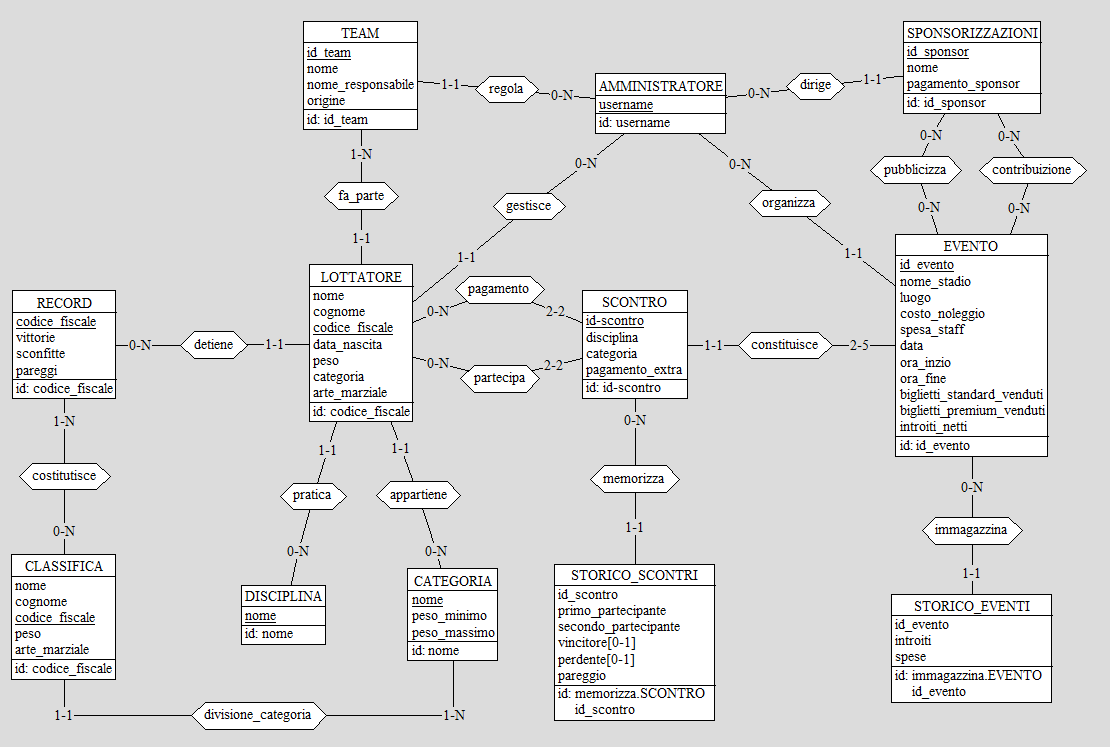
\includegraphics[scale=0.8, angle=90]{./img/schema_finale.png}

\chapter{Progettazione logica}
\section{Stima del volume dei dati}
\begin{itemize}
    \item AMMINISTRATORE: E, 1
    \item LOTTATORE: E, 250
    \item CATEGORIA: E, 4
    \item DISCIPLINA: E, 3
    \item RECORD: E, 250
    \item CLASSIFICA: E, 250
    \item SCONTRO: E, 2000
    \item STORICO\textunderscore SCONTRI: E, 2000
    \item EVENTO: E, 700
    \item STORICO\textunderscore EVENTI: E, 700
    \item SPONSORIZZAZIONI: E, 15
    \item TEAM: E, 150
    \item DIRIGE: A, 20
    \item GESTISCE: A, 350
    \item REGOLA: A, 200
    \item ORGANIZZA: A, 700
    \item DETIENE: A, 250
    \item CONSTITUISCE: A, 250
    \item MEMORIZZA: A, 2000
    \item DIVISIONE\textunderscore CATEGORIA: A, 4
    \item APPARTIENE: A, 250
    \item PRATICA: A, 375
    \item FA\textunderscore PARTE: A, 200
    \item PARTECIPA: A, 4000
    \item PAGAMENTO: A, 4000
    \item CONSTITUISCE: A, 2000
    \item PUBBLICIZZA: A, 3000
    \item CONTRIBUIZIONE: A, 3000
    \item IMMAGAZINA: A, 700
\end{itemize}

\section{Descrizione delle operazioni principali e stima della loro frequenza}
\begin{itemize}
    \item Registrazione nuovo lottatore: 1/10 g
    \item Rimuovere un lottatore: 1/15 g
    \item Registrazione nuovo team: 1/12 g
    \item Rimuovere un team: 1/18 g
    \item Registrare un nuovo sponsor: 1/120 g
    \item Rimuovere uno sponsor: 1/210 g
    \item Organizzare un evento: 1/30 g
    \item Visualizzare la classifica: 3/ g
    \item Modificare dati di un partecipante: 1/5 g
\end{itemize} 

\section{Schemi di navigazione e tabelle degli accessi}
\subsection{Registrazione nuovo lottatore}
\begin{table}[H]
    \paragraph{Tavola degli accessi\newline}
    \begin{tabular}{|c|c|c|c|}
    \hline
    Concetto          & Costrutto & Accessi & Tipo \\ \hline
    AMMINISTRATORE    & E         & 1       & R    \\ \hline
    LOTTATORE         & E         & 1       & W    \\ \hline
    GESTISCE          & A         & 1       & R    \\ \hline
    \textit{TOTALE}   &           & 4       &      \\ \hline
    \end{tabular}
\end{table}

\subsection{Rimuovere un lottatore}
\begin{table}[H]
    \paragraph{Tavola degli accessi\newline}
    \begin{tabular}{|c|c|c|c|}
    \hline
    Concetto          & Costrutto & Accessi & Tipo \\ \hline
    AMMINISTRATORE    & E         & 1       & R    \\ \hline
    LOTTATORE         & E         & 1       & W    \\ \hline
    GESTISCE          & A         & 1       & R    \\ \hline
    \textit{TOTALE}   &           & 4       &      \\ \hline
    \end{tabular}
\end{table}

\subsection{Registrazione/Rimozione nuovo team}
\begin{table}[H]
    \paragraph{Tavola degli accessi\newline}
    \begin{tabular}{|c|c|c|c|}
    \hline
    Concetto          & Costrutto & Accessi & Tipo \\ \hline
    AMMINISTRATORE    & E         & 1       & R    \\ \hline
    TEAM              & E         & 1       & W    \\ \hline
    REGOLA            & A         & 1       & R    \\ \hline
    \textit{TOTALE}   &           & 4       &      \\ \hline
    \end{tabular}
\end{table}

\subsection{Registrare/Rimuovere un nuovo sponsor}
\begin{table}[H]
    \paragraph{Tavola degli accessi\newline}
    \begin{tabular}{|c|c|c|c|}
    \hline
    Concetto          & Costrutto & Accessi & Tipo \\ \hline
    AMMINISTRATORE    & E         & 1       & R    \\ \hline
    SPONSORIZZAZIONI  & E         & 1       & W    \\ \hline
    DIRIGE            & A         & 1       & R    \\ \hline
    \textit{TOTALE}   &           & 4       &      \\ \hline
    \end{tabular}
\end{table}

\subsection{Organizzare un evento}
\begin{table}[H]
    \paragraph{Tavola degli accessi\newline}
    \begin{tabular}{|c|c|c|c|}
    \hline
    Concetto                         & Costrutto & Accessi & Tipo \\ \hline
    AMMINISTRATORE                   & E         & 1       & R    \\ \hline
    EVENTO                           & E         & 1       & W    \\ \hline
    SCONTRO                          & E         & 3       & W    \\ \hline
    SPONSORIZZAZIONI                 & E         & 1       & R    \\ \hline
    STORICO\textunderscore SCONTRI   & E         & 3       & W    \\ \hline
    STORICO\textunderscore EVENTI    & E         & 1       & W    \\ \hline
    LOTTATORE                        & E         & 6       & R    \\ \hline
    PARTECIPA                        & A         & 6       & R    \\ \hline
    CONSTITUISCE                     & A         & 3       & R    \\ \hline
    CONTRIBUIZIONE                   & A         & 1       & R    \\ \hline
    ORGANIZZA                        & A         & 1       & R    \\ \hline
    IMMAGAZINA                       & A         & 1       & R    \\ \hline
    STORICO\textunderscore SCONTRI   & A         & 3       & R    \\ \hline
    PAGAMENTO                        & A         & 1       & R    \\ \hline
    \textit{TOTALE}                  &           & 40      &      \\ \hline
    \end{tabular}
\end{table}

\subsection{Visualizzare la classifica}
\begin{table}[H]
    \paragraph{Tavola degli accessi\newline}
    \begin{tabular}{|c|c|c|c|}
    \hline
    Concetto                             & Costrutto & Accessi & Tipo \\ \hline
    CLASSIFICA                           & E         & 1       & R    \\ \hline
    CATEGORIA                            & E         & 1       & R    \\ \hline
    DIVISIONE\textunderscore CATEGORIA   & A         & 1       & R    \\ \hline
    \textit{TOTALE}                      &           & 3       &      \\ \hline
    \end{tabular}
\end{table}

\subsection{Modificare dati di un partecipante}
\begin{table}[H]
    \paragraph{Tavola degli accessi\newline}
    \begin{tabular}{|c|c|c|c|}
    \hline
    Concetto                         & Costrutto & Accessi & Tipo \\ \hline
    AMMINISTRATORE                   & E         & 1       & R    \\ \hline
    LOTTATORE                        & E         & 1       & W    \\ \hline
    RECORD                           & E         & 1       & W    \\ \hline
    CATEGORIA                        & E         & 1       & W    \\ \hline
    DISCIPLINA                       & E         & 1       & W    \\ \hline
    TEAM                             & E         & 1       & W    \\ \hline
    FA\textunderscore PARTE          & A         & 1       & R    \\ \hline
    PRATICA                          & A         & 1       & R    \\ \hline
    GESTISCE                         & A         & 1       & R    \\ \hline
    APPARTIENE                       & A         & 1       & R    \\ \hline
    DETIENE                          & A         & 1       & R    \\ \hline
    \textit{TOTALE}                  &           & 16      &      \\ \hline
    \end{tabular}
\end{table}

\end{document}
